%default language is German. use the second line instead for english settings:
\RequirePackage{ifpdf}
\documentclass{lni}
%\documentclass[english]{lni}

\IfFileExists{latin1.sty}{\usepackage{latin1}}{\usepackage{isolatin1}}

\usepackage{graphicx}
\usepackage[utf8]{inputenc}

% Extra packages

\usepackage{amsmath}
\usepackage{amssymb}
\usepackage{amsthm}

\usepackage{latexsym}

\usepackage{mathtools}

\usepackage{tikz}
\usetikzlibrary{automata,positioning}

\usepackage{turnstile}

\usepackage{algorithm}
\makeatletter
\renewcommand{\ALG@name}{Algorithmus}
\makeatother
\usepackage{algpseudocode}

% Own environments

\newtheoremstyle{def_style}
{\topsep}{\topsep}%
{}{}%
{\bfseries}{}%
{\newline}{}%

\theoremstyle{def_style}
\newtheorem{definition}{Definition}[section]

\newtheoremstyle{break}
{\topsep}{\topsep}%
{}{}%
{\bfseries}{}%
{\newline}{}%

\theoremstyle{break}
\newtheorem{example}{Beispiel}

% Own commands

\newcommand{\AU}[2]{\operatorname{A}[#1\operatorname{U}#2]}
\newcommand{\EU}[2]{\operatorname{E}[#1\operatorname{U}#2]}

\newcommand{\UEqual}[4]{#1\operatorname{U}^{\leq #2}_{\geq #3}#4}
\newcommand{\UStrict}[4]{#1\operatorname{U}^{\leq #2}_{> #3}#4}
\newcommand{\WeakEqual}[4]{#1\operatorname{\mathcal{U}}^{\leq #2}_{\geq #3}#4}
\newcommand{\WeakStrict}[4]{#1\operatorname{\mathcal{U}}^{\leq #2}_{> #3}#4}

\newcommand{\paths}[2]{\operatorname{paths}^{#1}_{#2}}

\newcommand{\Arrow}[4]{#1 \leadsto^{\leq #2}_{\geq #3}#4}


\author{
	Theodor Teslia \\ 
	\\ 
	Informatik 11 -- Embedded Software \\ 
	RWTH Aachen University \\ 
	Aachen, Germany \\ 
	teslia@embedded.rwth-aachen.de\\
	\\
	\textit{Betreuer}\\
	\textit{Robin Mross}\\ %Dies ist der inhaltliche Betreuer. Wer das ist, erfahren Sie noch.
}
\title{\small{Seminar} \\ \vspace{0.5cm} \Large{Eine Logik für das Schlussfolgern über Zeit und Zuverlässigkeit}}

\newcommand{\CTL}{\mathsf{CTL}}
\newcommand{\PCTL}{\mathsf{PCTL}}

\begin{document}
\maketitle

\begin{abstract}
Eine prägnante Zusammenfassung des Kerninhaltes ohne thematische Einleitung und Fazit. Was ist $\PCTL$ und welche Probleme kann es lösen, die andere Logiken bisher nicht erfüllen konnten.
\end{abstract}

\section{Einführung}

Hier führe ich in die Logik $\PCTL$ ein, die Probleme die diese löst und wie dies circa gemacht wird.
Falls es funktioniert, führe ich außerdem in Halbringsemantik ein und erkläre kurz, in welchem Punkt sich die Ansätze ähneln und unterscheiden.

\section{Grundlagen}
\label{ChapGrundlagen}

Um Erweiterungen einer Logik zu verstehen ist es ratsam die Grundlegende auch zu kennen. Aus diesem Grund soll in diesem Kapitel in die Logik \textit{Computation Tree Logic} ($\CTL$) und naheliegende, wichtige Themen eingeleitet werden.

$\CTL$ ist eine temporale Logik um Aussagen in nicht-deterministischen Systemen zu treffen. 
Dafür betrachtet man Kripkestrukturen, welche eine Art Graph darstellen, da diese viele Eigenschaften liefern, die für $\CTL$-Anwendungsfälle interessant sind.

\begin{definition}[Syntax von $\CTL$]
	Die Menge der $\CTL$-Formeln lässt sich induktiv mithilfe folgender Regeln definieren \cite{clarke1982design, baier2008principles}:
	\begin{enumerate}
		\item Wenn $\mathsf{AP}$ eine Menge an atomaren Aussagen ist, dann ist jedes $a\in \mathsf{AP}$ eine $\CTL$-Formel. Außerdem sind $\top$ und $\bot$ $\CTL$-Formeln.
		\item Wenn $\varphi_1$ und $\varphi_2$ $\CTL$-Formeln sind, dann sind $\neg\varphi_1$, $\varphi_1 \land \varphi_2$ und $\varphi_1 \lor \varphi_2$ ebenfalls $\CTL$-Formeln.
		\item Wenn $\varphi_1$ eine $\CTL$-Formel ist, dann sind auch $\operatorname{EX}\varphi_1$ und $\operatorname{AX}\varphi_1$ $\CTL$-Formeln.
		\item Wenn $\varphi_1$ und $\varphi_2$ $\CTL$-Formeln sind, dass sind $\EU{\varphi_1}{\varphi_2}$ und $\AU{\varphi_1}{\varphi_2}$ auch $\CTL$-Formeln.
	\end{enumerate}
\end{definition}

Bevor die Semantik erläutert wird, sollen zuerst die Strukturen gezeigt werden, die man typischerweise mit $\CTL$ zusammen verwendet.

\begin{definition}[Kripkestrukturen]
	Eine \textit{Kripkestruktur} oder \textit{Transitionssystem} ist ein Graph von der Form $\mathcal{K}=(V, E, \mathcal{L})$, wobei $E$ eine zweistellige Kantenrelation über $V$ ist und $\mathcal{L}$ eine Funktion $\mathcal{L}:V\to2^{\mathsf{AP}}$ ist, die jedem Zustand eine Menge an atomaren Aussagen zuweist 	\cite{clarke1982design,clarke1986automatic}.
	
	Weiter bezeichnen wir einen Pfad als $\sigma=s_0\dots s_n$ mit $s_i\in V$ für alle $i\in\{0,\dots,n\}$ und $\sigma[i]=s_i$ für $0\leq i \leq n$ \cite{baier2008principles}.
\end{definition}

\begin{definition}[Semantik von $\CTL$]
	Für ein Transitionssystem $\mathcal{K}=(V,E,\mathcal{L})$ können wir damit induktiv die Modellbeziehung $\models$ zwischen einem Knoten $v\in V$ und $\CTL$-Formeln definieren \cite{baier2008principles}:
	\begin{enumerate}
		\item $v\models \top \Leftrightarrow \mathcal{K}\models\forall x(x=x)$ und $v\models \bot \Leftrightarrow \mathcal{K}\models\exists x(x\neq x)$.
		\item Für $a\in \operatorname{AP}$ gilt $v\models a \Leftrightarrow a\in \mathcal{L}(v)$.
		\item Es gilt $v\models \neg \varphi \Leftrightarrow v\not\models \varphi$,\\
		$v\models \varphi_1 \land \varphi_2 \Leftrightarrow v\models \varphi_1 \text{ und } v\models \varphi_2$,\\
		$v\models \varphi_1 \lor \varphi_2 \Leftrightarrow v\models \varphi_1 \text{ oder } v\models \varphi_2$,
		\item Es gilt $v\models \operatorname{EX}\varphi \Leftrightarrow$ es ex. ein $w\in V$ mit $(v,w)\in E$ und $w\models \varphi$ und analog:\\ 
		$v\models \operatorname{AX}\varphi \Leftrightarrow$ für alle $w\in V$ mit $(v,w)\in E$ gilt $w\models \varphi$.
		\item Es gilt $v\models \EU{\varphi_1}{\varphi_2} \Leftrightarrow$ es existiert ein Pfad $\sigma$ in $\mathcal{K}$, der in $v$ beginnt und ein $i\in \mathbb{N}$ so, dass $\sigma[i]\models \varphi_2$ und für alle $0\leq j < i$ gilt $\sigma[i]\models \varphi_1$. 
		Analog ist die Definition für $\AU{\varphi_1}{\varphi_2}$, es muss dann aber für jeden in $v$ beginnenden Pfad ein $i\in \mathbb{N}$ geben so, dass der $i$-te Zustand $\varphi_2$ und alle Zustände davor $\varphi_1$ erfüllen.
	\end{enumerate}
\end{definition}

Intuitiv bedeutet $\operatorname{EX}\varphi$ also, dass $\varphi$ in einem beliebigen Nachfolgezustand gelten muss und $\operatorname{AX}\varphi$, dass $\varphi$ von allen Nachfolgezuständen erfüllt wird.

$\EU{\varphi_1}{\varphi_2}$ bzw. $\AU{\varphi_1}{\varphi_2}$ sagt aus, dass es einen Pfad $\sigma$ gibt bzw. auf allen Pfaden $\sigma$ gilt, dass zuerst $\varphi_1$ gilt, bis von einem Zustand $\varphi_2$ erfüllt wird.
Die anderen Operatoren haben die bekannte Bedeutung.

Um einige Eigenschaften einfacher auszudrücken werden zusätzlich noch weitere Operatoren definiert \cite{clarke1982design}:
\begin{itemize}
	\item $\operatorname{EF}\varphi \equiv \EU{\top}{\varphi}$ und $\operatorname{AF}\varphi \equiv \AU{\top}{\varphi}$ bedeuten intuitiv, dass es einen Pfad gibt bzw. für alle Pfade irgendwann $\varphi$ gilt.
	\item $\operatorname{EG}\varphi \equiv \neg\operatorname{EF}\neg\varphi$ und $\operatorname{AG}\varphi \equiv \neg\operatorname{AF}\neg\varphi$ bedeuten, dass es einen Pfad gibt bzw. für alle Pfade gilt, dass in jedem Zustand $\varphi$ gilt.
\end{itemize}
Mithilfe dieser Syntax und zugehöriger Semantik auf Transitionssystemen lassen sich nun einige interessante Aussagen formulieren:
\begin{example}[Beispiele für $\CTL$-Formeln und deren Bedeutung]
	Sei die Menge der atomaren Aussagen $\mathsf{AP}=\{\mathsf{idle}, \mathsf{error}\}$
	\begin{itemize}
		\item $\operatorname{AG}\operatorname{AF}\mathsf{idle}$ \\ Die Formel gilt für einen Zustand $v$, wenn auf jedem in $v$ beginnenden Pfad, für jeden Zustand auf diesem, irgendwann $\mathsf{idle}$ erfüllt. Das heißt, $\mathsf{idle}$ gilt unendlich oft.
		\item $\operatorname{EF}\operatorname{AG}\mathsf{error}$ \\
		Diese $\CTL$-Formel besagt, dass es einen Pfad gibt, auf dem ab irgendeinem Zustand alle Zustände die atomare Aussage $\mathsf{error}$ erfüllen. Das heißt, es gibt einen Pfad mit einem irreversiblen Fehler.
	\end{itemize}
\end{example}

Zusätzlich soll noch angemerkt werden, dass $0\in \mathbb{N}$ gilt.

\section{Eine Logik für Zeit und Zuverlässigkeit}

% Dieses Kapitel stellt das Hauptkapitel der Arbeit dar und soll die Syntax und Semantik von $\PCTL$ erläutern, sowie mithilfe von eigenen Beispielen diese Verständlicher machen. Offensichtliche verwende ich in dem gesamten Kapitel hauptsächlich \cite{hansson1994logic} für Informationen, Algorithmen und Beweise, die Beispiele werden aber zum Großteil eigene sein.

Wie in Kapitel \ref{ChapGrundlagen} gezeigt, lassen sich mithilfe von $\CTL$ viele interessante Eigenschaften von nicht-deterministischen System beschreiben. 
Jedoch gibt es auch Anwendungsfälle, in denen mehr Ausdruckskraft benötigt wird, als ein All- und Existenzquantor liefern können.
Ein Gebiet in dem dies stark auffällt sind Soft-Realtime Systeme. 
In diesen existieren für Prozesse bestimmte Zeitschranken (\textit{Deadlines}), im Gegensatz zu Hard-Realtime Systemen führt das einhalten einer Zeitschranke aber nicht zu einem Systemabbruch oder katastrophalem Ereignis, sondern stellt beispielsweise nur eine Verschlechterung der Effizienz dar. \cite{hansson1994logic}.
Um eben solche Systeme gut beschreiben zu können benötigt man zwei weitere Aspekte:
\begin{enumerate}
	\item Um die Zeitschranken zu formulieren wird ein Konzept von Zeit benötigt. Dieses soll aussagen können, dass zwei Ereignisse eine bestimmte Zeitspanne $t$ voneinander entfernt sind.
	\item Da aber das Verfehlen einer Zeitschranke nicht unbedingt zum Verwerfen einer Formel führen soll, werden zusätzlich Wahrscheinlichkeiten benötigt. 
	Da in Soft-Realtime Systemen das Überschreiten einer Deadline zwar nicht direkt verboten ist, aber im Allgemeinen vermieden werden sollte, ist es sinnvoll über die Wahrscheinlichkeit eines Ereignisses Aussagen zu treffen.
\end{enumerate}
Kombiniert man diese Aspekte lassen sich Eigenschaften wie \glqq Nach Ereignis X passiert innerhalb von 15 Zeiteinheiten mit Wahrscheinlichkeit 90\% Ereignis Y\grqq{} oder \glqq Ereignis A tritt mit einer Wahrscheinlichkeit von 90\% in 10 und mit 95\% in 20 Zeitschritten auf\grqq. 
Eine Logik, die eben diese Erweiterungen von $\CTL$ sinnvoll implementiert ist die Logik \text{Probabilistic Computation Tree Logic} ($\PCTL$). 
Sinnvoll bedeutet hier, dass es einen Model Checking Algorithmus mit polynomieller Laufzeit gibt. 
In diesem Kapitel soll zuerst die Syntax von $\PCTL$ erläutert werden, danach die dazugehörige Semantik aufgezeigt werden, um dann zwei verschiedene Ansätze für das Model Checking von $\PCTL$ mit Transitionssystemen zu zeigen. 
Im Anschluss sollen die kennengelernten Konzepte der Logik sowie des Model Checkings an einem Beispiel erläutert werden.

\subsection{Syntax und Semantik von $\PCTL$}

Um \textit{Probabilistic Computation Tree Logic} ($\PCTL$) besser zu verstehen, soll hier die Syntax, die Modelle welche wir zum Auswerten verwenden, sowie die Semantik der Logik erläutert werden.

Wie auch für $\CTL$ können wir die Syntax von  $\PCTL$ mithilfe folgender rekursiver Regeln definieren:
\begin{definition}[Syntax von $\PCTL$]
	\label{SyntaxPCTL}
	Die Menge der $\PCTL$-Formeln lässt sich induktiv wie folgt definieren \cite{hansson1994logic}:
	\begin{enumerate}
		\item Es gilt $\top\in \PCTL$ und $\bot\in \PCTL$.
		\item Wenn $\mathsf{AP}$ die Menge atomarer Aussagen ist, dann ist jedes $a\in \mathsf{AP}$ eine $\PCTL$ Formel.
		\item Wenn $\varphi_1$ und $\varphi_2$ $\PCTL$-Formeln sind, dann sind $\neg\varphi_1$ und $(\varphi_1\land \varphi_2)$ auch $\PCTL$-Formeln.
		\item Für zwei $\PCTL$-Formeln $\varphi_1$ und $\varphi_2$, $t\in \mathbb{N}\cup\{\infty\}$ und $p\in [0,1]\subseteq\mathbb{R}$, sind $\UEqual{\varphi_1}{t}{p}{\varphi_2}$ und $\UStrict{\varphi_1}{t}{p}{\varphi_2}$ auch $\PCTL$-Formeln.
	\end{enumerate}
\end{definition}
Mit diesen Regeln können wir einige $\PCTL$-Formeln aufstellen.
\begin{example}[Korrekte und inkorrekte $\PCTL$-Formeln]
	Sei $\mathsf{AP}=\{A,B,X,Y\}$. Dann wären 
	$$\neg(X \land \neg(\UEqual{\top}{15}{90\%}{Y})) \text{ und } (\UEqual{A}{10}{90\%}{B}) \land (\UStrict{A}{20}{95\%}{B})$$ 
	korrekte $\PCTL$-Formeln.
	
	Inkorrekt gebildete Formeln wären zum Beispiel $$\neg(X \land \neg(\UEqual{\top}{15}{90\%}{})) \text{ und } (\UEqual{A}{10}{90\%}{B})(\UStrict{A}{20}{95\%}{B}).$$
\end{example}

Ähnlich, wie wir Transitionssysteme definiert haben, um diese als Modelle von $\CTL$-Formeln zu verwenden, wollen wir nun sogenannte Markov-Ketten definieren, um Eigenschaften von diesen mithilfe von $\PCTL$ zu formulieren.

\begin{definition}[Markov-Ketten]
	Sei $S$ eine endliche Menge, $s_i\in S$ und $\mathcal{L}:S\to 2^\mathsf{AP}$ sowie $\mathcal{T}:S\times S \to [0,1]$ Funktionen so, dass für alle $s\in S$ gilt: $\sum_{s'\in S}\mathcal{T}(s,s')=1$.
	
	Dann nennen wir $\mathfrak{S}=(S, s_i, \mathcal{T}, \mathcal{L})$ eine Markov-Kette, wobei $S$ eine Menge an Zuständen ist, $s_i$ der Anfangszustand, $\mathcal{T}$ die Transitions-Wahrscheinlichkeits-Funktion und $\mathcal{L}$ die Bezeichnungsfunktion, die jedem Zustand eine Menge an atomaren Aussagen zuweist.
	
	Weiter bezeichnen wir mit $\paths{\mathfrak{S}}{s_0}$ die Menge der Pfade in $\mathfrak{S}$, die in $s_0$ beginnen. 
	Ein $\sigma\in \paths{\mathfrak{S}}{s_0}$ ist dann von der Form $\sigma=s_0s_1s_2\dots$ und wir definieren $\sigma[n]\coloneqq s_n$ als den $n$-ten Zustand des Pfads und $\sigma\uparrow n\coloneqq s_0\dots s_n$ als den $n+1$ langen Präfix des Pfads.
	\cite{hansson1994logic}
\end{definition}

Zur Einfachheit sagen wir, dass zwischen vom Knoten $s$ zum Knoten $s'$ genau dann eine Kante existiert, wenn $\mathcal{T}(s, s') \neq 0$.
Man erkennt, dass im Allgemeinen ein Pfad $\sigma\in \paths{\mathfrak{S}}{s_0}$ unendlich lang ist. 
Dies ist wohldefiniert, da jeder Zustand eine ausgehende Kante haben muss. Andernfalls gibt es ein $\hat s\in S$ mit $\{s'\in S :\mathcal{T}(\hat s, s')= 0 \} = S$. Aber dann ist $\sum_{s'\in S}\mathcal{T}(\hat s, s')=0$. Widerspruch! Es gibt für jeden Zustand also mindestens einen Nachfolgezustand, es gibt also immer unendliche Pfade.

Eine Markov Kette ist also ein gerichteter, gewichteter Graph, wobei die Gewichtung der Kanten angibt, wie wahrscheinlich es ist, eine bestimmte Kante auszuwählen. Zusätzlich soll die Summe aller Gewichte der ausgehenden Kanten eines Knotens immer gleich eins sein. Damit ist auch gewährleistet, dass es keine isolierten Knoten gibt.

Im Kontext von Systemen sollen die Zustände des Graphens Zustände des Systems beschreiben. Die Kanten stellen die Möglichen Folgezustände des Systems dar, wobei der Wechsel in einen Folgezustand mit der Wahrscheinlichkeit durchgeführt wird, mit der die Kante annotiert ist. In jedem Zustand gelten atomare Aussagen, welche die Zustände beschreiben, diese werden von der Funktion $\mathcal{L}$ zugewiesen.

Betrachten wir eine Markov-Kette als Beispiel:
\begin{example}[Beispiel einer Markov-Kette]
	Sei $S=\{s_0,s_1, s_2\}$, $\mathcal{L}=\{s_0\mapsto \{A\}, s_1\mapsto \{A,B\}, s_2 \mapsto \{C\}\}$ und $\mathcal{T}$ durch Tabelle \ref{MarkovT1} definiert. Dann ist $\mathfrak{S}=(S,s_0,\mathcal{T},\mathcal{L})$ die in Abbildung \ref{MarkovGraph1} graphisch dargestellte Markov-Kette, wobei Transitionen mit einer Wahrscheinlichkeit von $0$ nicht eingezeichnet werden.
	
	\begin{table}[h]
		\begin{center}
			\begin{tabular}{c|ccc}
				$\mathcal{T}$ & $s_0$ & $s_1$ & $s_2$ \\
				\hline
				$s_0$ & $0$  & $0.7$ & $0.3$ \\
				$s_1$ & $0.8$ & $0$   & $0.2$ \\
				$s_2$ & $0$  & $0$  & $1$   \\
			\end{tabular}
			\caption{Tabelle zur Definition der Funktion $\mathcal{T}:S\times S\to [0,1]$}
			\label{MarkovT1}
		\end{center}
	\end{table}
	
	\begin{figure}[h]
		\begin{center}
			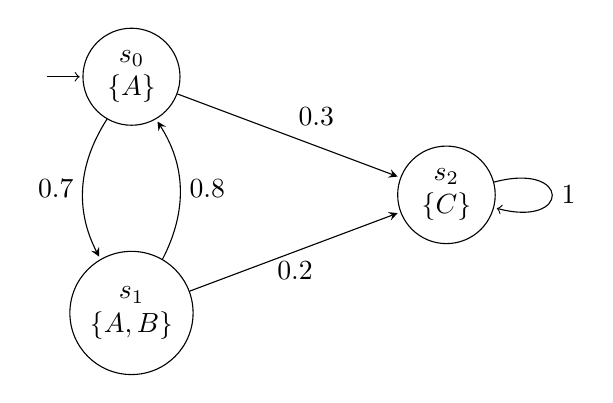
\begin{tikzpicture}[shorten >= 1pt, node distance=4cm, on grid, auto]
				\node[state, initial, initial text={}, align=center] (s_0) [] {$s_0$ \\ $\{A\}$};
				\node[state, align=center] (s_1) [below=of s_0, yshift=1cm] {$s_1$ \\ $\{A,B\}$};
				\node[state, align=center] (s_2) [right=of s_0, yshift=-1.5cm] {$s_2$ \\ $\{C\}$};
				
				\path[-stealth]
				(s_0) edge [bend right] node[left] {$0.7$} (s_1)
				(s_0) edge [] node {$0.3$} (s_2)
				(s_1) edge [bend right] node[right] {$0.8$} (s_0)
				(s_1) edge [] node[below] {$0.2$} (s_2)
				(s_2) edge [loop right] node {$1$} (s_2)
				;
			\end{tikzpicture}
			
			\caption{Graph für die Markov-Kette $\mathfrak{S}$}
			\label{MarkovGraph1}
		\end{center}
	\end{figure}
\end{example}

Bevor wir die Semantik von $\PCTL$-Formeln für Markov-Ketten formal definieren können benötigen wir noch den Begriff des Wahrscheinlichkeitsmaßes.

\begin{definition}[Wahrscheinlichkeitsmaß]
	 Sei $\pi = s_0\dots s_n$ eine Folge an Zuständen einer Markov-Kette $\mathfrak{S}$ und $X=\{\sigma\in \paths{\mathfrak{s}}{s_0} : \sigma\uparrow n = \pi\}$ die Menge aller (unendlichen) Pfade, die mit dieser Folge beginnen. Wir definieren dann das Wahrscheinlichkeitsmaß 
	 $$\mu^{\mathfrak{S}}_{s_0}(X)\coloneqq\mathcal{T}(s_0,s_1)\cdot \dots \cdot \mathcal{T}(s_{n-1},s_n),$$
	 als das Produkt der Kanten zwischen den Zustände der Folge. \cite{hansson1994logic}
\end{definition}

Weiter ergeben sich einige Gleichheiten \cite{hansson1994logic}:
\begin{itemize}
	\item Wählt man eine leere Folge mit Länge ergibt sich
	\begin{equation}\mu^\mathfrak{S}_{s_0}(\{\sigma\in \paths{\mathfrak{S}}{s_0} : \sigma\uparrow 0 = s_0\})=1.\end{equation}
	\item Für eine abzählbare Menge $(X_i)_{i\in I}$ mit paarweise disjunkten Mengen an Pfaden gilt
	\begin{equation}\mu^\mathfrak{S}_{s_0}(\bigcup_{i\in I}X_i) = \sum_{i\in I}\mu^\mathfrak{S}_{s_0}(X_i).\end{equation}
	\item Sei $X\subseteq \paths{\mathfrak{S}}{s_0}$ dann folgt 
	\begin{equation}\mu^\mathfrak{S}_{s_0}(\paths{\mathfrak{S}}{s_0} \setminus X) = 1-\mu^\mathfrak{S}_{s_0}(X).\label{MassUmkehrung}\end{equation}
\end{itemize}

Betrachten wir zum verdeutlichen ein paar Beispiele.
\begin{example}[Wahrscheinlichkeitsmaße]
	Der Einfachheit halber verwenden wir wieder die Markov-Kette aus Abbildung \ref{MarkovGraph1}. Sei $\pi=s_0s_1s_0s_2$. 
	Dann ist $X=\{\sigma \in \paths{\mathfrak{S}}{s_1} : \sigma\uparrow 3 = \pi\}$ die Menge der Pfade, die durch folgenden Ausdruck dargestellt werden: $s_0s_1s_0(s_2)^\omega$ und es folgt
	$$\mu^\mathfrak{S}_{s_0}(X)=\mathcal{T}(s_0,s_1) \cdot \mathcal{T}(s_1,s_0) \cdot \mathcal{T}(s_0,s_2) = 0.7 \cdot 0.8 \cdot 0.3 = 0.168$$
	
	Als zweites Beispiel wollen wir alle Pfade betrachten, die dem Ausdruck $s_0(s_1s_0)^\ast s_2$ entsprechen. Also alle Pfade, die endlich oft zwischen $s_0$ nach $s_1$ und wieder zurück wechseln und dann in $s_4$ enden. Es gilt:
	\begin{align*}
		\mu^\mathfrak{S}_{s_0}&(\{\sigma\in \paths{\mathfrak{S}}{s_0} : \exists i\in \mathbb{N} (\sigma\uparrow 2i+1 = s_0(s_1s_0)^i s_2)\}) \\
		&=\mu^\mathfrak{S}_{s_0} \left(\bigcup_{i\in \mathbb{N}} \{\sigma\in \paths{\mathfrak{S}}{s_0} : \sigma\uparrow 2i+1 = s_0(s_1s_0)^i s_2\}\right) \\
		&=\sum_{i\in \mathbb{N}} \mu^\mathfrak{S}_{s_0}(\{\sigma\in \paths{\mathfrak{S}}{s_0} : \sigma\uparrow 2i+1 = s_0(s_1s_0)^i s_2\}) \\
		&=\sum_{i\in \mathbb{N}} (\mathcal{T}(s_0, s_1) \cdot \mathcal{T}(s_1, s_0))^i \cdot \mathcal{T}(s_0,s_2) \\
		&=\sum_{i\in \mathbb{N}} 0.56^i \cdot 0.3 = 0.3 \cdot \sum_{i\in \mathbb{N}} 0.56^i \\
		&= 0.3 \cdot \frac{1}{1-0.56} \approx 0,6818
	\end{align*}
	
	Zuletzt soll ausgerechnet werden wie hoch die Wahrscheinlichkeit ist, niemals $s_2$ zu erreichen. Dies sind die genau die Pfade, die nur zwischen $s_0$ und $s_1$ hin-und-her wechseln. Ein alternativer Weg ist es, das Wahrscheinlichkeitsmaß der Pfade zu berechnen, die endlich von zwischen $s_0$ und $s_1$ wechseln und dann von $s_1$ aus in $s_2$ enden, also dem Ausdruck $s_0s_1(s_0s_1)^\ast s_2$ entsprechen. Die Berechnung verläuft analog zu dem eben vorgeführten Beispiel. Das Ergebnis ist dann $0.14\cdot\frac{1}{1-0.56} \approx 0.3182$. Es fällt auf, dass die Summe der letzten beiden Werte $1$ ist. Fasst meine beide Berechnungen zusammen erhält man demnach, dass die Wahrscheinlichkeit endlich oft zwischen $s_0$ und $s_1$ zu wechseln und irgendwie in $s_2$ zu enden gleich $1$ ist. Mit Gleichung \ref{MassUmkehrung} ist die Wahrscheinlichkeit nie in $s_2$ zu enden also $0$.
\end{example}

Nun können wir die Semantik von $\PCTL$ definieren. Genauer definieren wir eine Relation $\models_\mathfrak{S}$ für eine Markov-Kette $\mathfrak{S}=(S,s_i,\mathcal{T},\mathcal{L})$, ein $s\in S$ und eine $\PCTL$-Formel $\varphi$. Zur Vereinfachung definieren wir noch die Relation $\sttstile{}{}_\mathfrak{S} \subseteq \paths{\mathfrak{S}}{s} \times X$, wobei $X$ die Menge der Ausdrücke von der Form $\varphi_1 \operatorname{U}^{\leq t}\varphi_2$ mit $\varphi_1,\varphi_2 \in \PCTL, t\in \mathbb{N}$ ist.  

\begin{definition}[Semantik von $\PCTL$ auf Markov-Ketten]
	Sei $\mathfrak{S}=(S,s_i,\mathcal{T},\mathcal{L})$ eine Markov-Kette und $s_0\in S$. Dann lässt sich die Semantik für $\PCTL$-Formeln induktiv definieren \cite{hansson1994logic}:
	\begin{enumerate}
		\item $s_0 \models_\mathfrak{S} \top \Leftrightarrow \mathfrak{S}\models \forall x(x=x)$ und $s_0\models_\mathfrak{S} \bot \Leftrightarrow \mathfrak{S}\models \exists x(x\neq x)$
		\item Für $a\in \mathsf{AP}$ gilt $s_0\models_\mathfrak{S} a \Leftrightarrow a\in \mathcal{L}(s_0)$
		\item $s_0 \models_\mathfrak{S}\neg \varphi \Leftrightarrow \text{ nicht} s_0\models_\mathfrak{S} \varphi$
		\item $s\models_\mathfrak{S} \varphi_1\land\varphi_2 \Leftrightarrow s_0\models_\mathfrak{S} \varphi \text{ und } s_0\models_\mathfrak{S} \varphi_2$
		\item $\sigma \sttstile{}{} \varphi_1\operatorname{U}^{\leq t}\varphi_2 \Leftrightarrow \exists i\leq t(\sigma[i]\models_\mathfrak{S} \varphi_2 \text{ und } \sigma[j]\models_\mathfrak{S} \varphi_1 \text{ für alle } 0 \leq j<i)$
		\item $s_0\models_\mathfrak{S} \UEqual{\varphi_1}{t}{p}{\varphi_2} \Leftrightarrow \mu^\mathfrak{S}_{s_0}(\{\sigma \in \paths{\mathfrak{S}}{s_0} : \sigma \sttstile{}{}\varphi_1\operatorname{U}^{\leq t}\varphi_2\})\geq p$
		\item $s_0\models_\mathfrak{S} \UStrict{\varphi_1}{t}{p}{\varphi_2} \Leftrightarrow \mu^\mathfrak{S}_{s_0}(\{\sigma \in \paths{\mathfrak{S}}{s_0} : \sigma \sttstile{}{}\varphi_1\operatorname{U}^{\leq t}\varphi_2\}) > p$
	\end{enumerate}
\end{definition}

Es fällt auf, dass im Operator $\UEqual{}{t}{p}{}$, der Parameter $t$  Zeiteinheiten beschreibt, wobei eine Zeiteinheit genau eine Transition in der Markov-Kette ist. Analog beschreibt $p$ die Wahrscheinlichkeit, dass ein gültiger Pfad \glqq genommen\grqq{} wird.

Zusätzlich können wir weitere Operatoren definieren, um Formeln zu vereinfachen.
Wie bekannt sind $\neg$ und $\land$ funktional vollständig, weshalb wir die bekannten booleschen Operatoren wie folgt definieren können:
\begin{itemize}
	\item $\varphi_1 \lor \varphi_2 \equiv \neg(\neg\varphi_1 \land \neg\varphi_2)$
	\item $\varphi_1 \rightarrow \varphi_2 \equiv \neg\varphi_1 \lor \varphi_2$.
\end{itemize}
Zusätzlich definieren wir den \textit{außer} Operator $\mathcal{U}$ \cite{hansson1994logic}:
\begin{itemize}
	\item $ \WeakEqual{\varphi_1}{t}{p}{\varphi_2} \equiv \neg(\UStrict{\neg\varphi_1}{t}{1-p}{\neg(\varphi_1\lor\varphi_2)})$
	\item $ \WeakStrict{\varphi_1}{t}{p}{\varphi_2} \equiv \neg(\UEqual{\neg\varphi_1}{t}{1-p}{\neg(\varphi_1\lor\varphi_2)})$.
\end{itemize}
Intuitiv bedeutet $\varphi_1 \mathcal{U}^{\leq t}_{\geq p}\varphi_2$, dass mit einer Wahrscheinlichkeit von mindestens $p$ entweder $\varphi_1$ für $t$ Zeiteinheiten gilt, oder innerhalb von $t$ Zeiteinheiten $\varphi_2$ erfüllt wird und bis dahin $\varphi_1$ gilt. Die Bedeutung von $\varphi_1 \mathcal{U}^{\leq t}_{>p}\varphi_2$ ist analog. \cite{hansson1994logic}

Bevor wir nun Beispiele betrachten wollen, soll noch ein Vergleich mit $\CTL$ stattfinden, welcher uns zusätzliche, sehr nützliche Operatoren liefern wird. 
Wie in Kapitel \ref{ChapGrundlagen} erläutert wurde, besitzt $\CTL$ weder Aussagen über Zeit, noch Wahrscheinlichkeiten. 
Demnach können wir a priori einschränken, dass $t=\infty$ gelten muss und $p\in\{0,1\}$, abhängig davon, ob ein $\operatorname{A}$ oder $\operatorname{E}$ verwendet wird.
Man kann folgende Äquivalenzen finden \cite{hansson1994logic}:
\begin{itemize}
	\item $\AU{\varphi_1}{\varphi_2} \equiv \UEqual{\varphi_1}{\infty}{1}{\varphi_2}$
	\item $\EU{\varphi_1}{\varphi_2} \equiv \UStrict{\varphi_1}{\infty}{0}{\varphi_2}$
	\item $\operatorname{AF}\varphi \equiv \UEqual{\top}{\infty}{1}{\varphi}$
	\item $\operatorname{EF}\varphi \equiv \UStrict{\top}{\infty}{0}{\varphi}$
	\item $\operatorname{AG}\varphi \equiv \WeakEqual{\varphi}{\infty}{1}{\bot}$
	\item $\operatorname{EG}\varphi \equiv \WeakStrict{\varphi}{\infty}{0}{\bot}$
\end{itemize}
Intuitiv haben die Operatoren die aus Kapitel \ref{ChapGrundlagen} bekannten Bedeutungen.
Durch die Fähigkeiten von $\PCTL$ lassen sich die vier unären Operatoren verallgemeinern. 
Betrachtet man die Formeln $\operatorname{G}^{\leq t}_{\geq p}\varphi \equiv \WeakEqual{\varphi}{t}{p}{\bot}$ und $\operatorname{F}^{\leq t}_{\geq p}\varphi \equiv \UEqual{\top}{t}{p}{\varphi}$ fällt einem auf, dass diese eben die Bedeutung von $\operatorname{EG}/\operatorname{AG}$ und $\operatorname{EF}/\operatorname{AF}$ für arbiträre $t\in \mathbb{N}\cup\{\infty\}$ und $p\in [0,1]$ ausweiten. 
$\operatorname{G}^{\leq t}_{\geq p}\varphi$ gilt also genau dann, wenn die Wahrscheinlichkeit, dass $\varphi$ für $t$ Zeiteinheiten mindestens $p$ ist und $\operatorname{F}^{\leq t}_{\geq p}\varphi$ bedeutet, dass mit einer Wahrscheinlichkeit von $p$, $\varphi$ innerhalb von $t$ Zeiteinheiten gelten wird. \cite{hansson1994logic}

In der Beschreibung von Systemen sind bedingte Aussagen wie zum Beispiel \glqq Wenn $A$ passiert, wird $B$ passieren\grqq{} sehr hilfreich. Daher soll ein Operator, der solch ein Verhalten, verbunden mit Zeit- und Wahrscheinlichkeitsparametern, für $\PCTL$ definiert werden:
$$\Arrow{\varphi_1}{t}{p}{\varphi_2} \equiv \operatorname{AG}(\varphi_1\rightarrow\operatorname{F}^{\leq t}_{^geq p} \varphi_2),$$
mit der intuitiven Bedeutung, dass wenn $\varphi_1$ gilt, dann wird mit einer Wahrscheinlichkeit von mindestens $p$, in $t$ Schritten $\varphi_2$ erfüllt. \cite{hansson1994logic}

Nun können wir Ausdrücke formulieren, die interessante Eigenschaften von Systemen beschreiben. Beginnen wir zuerst mit einigen abstrakten Beispielen.
\begin{example}[Abstrakte Beispiele für $\PCTL$-Formeln]
	\label{PCTLBeispiel}
	Wir betrachten wieder die Markov-Kette aus Abbildung \ref{MarkovGraph1}.
	% Eif nur genannte Beispiele von vorher aufgreifen
	% Sachen mit den schon berechneten Wahrscheinlichkeitsmaßen machen -> Nicht erreichen von s_3 ist nicht möglich für unendliche Pfade
\end{example}

Die wir nun vertraut mit der Funktionsweise von $\PCTL$ sind, wollen wir das algorithmische Lösen des Model-Checking Spiels für $\PCTL$-Formeln und Markov-Ketten betrachten.

\subsection{Das Model-Checking Spiel für $\PCTL$}

Ein wichtiges Anwendungsgebiet für temporale Logiken wie $\CTL$ und $\PCTL$ ist die Verifikation von Systemen. 
Bei diesem erhält man eine Struktur $\mathfrak{S}$ (im Fall von $\PCTL$ eine Markov-Kette) und eine $\PCTL$-Formel $\varphi$, welche das gewünschte Verhalten eines Systems beschreibt. 
Nun überprüft man ob $\mathfrak{S}\models \varphi$ gilt und falls dies der Fall ist, wurde somit gezeigt, dass das durch $\mathfrak{S}$ modellierte System sich korrekt verhält.
Da komplexe Systeme aber nur durch sehr große Strukturen modelliert werden können und sich kompliziertes Verhalten auch nicht mit kurzen Formeln dargestellt werden kann, ist es sinnvoll dieses Modellierungsproblem zu automatisieren, indem man Model Checking Algorithmen entwickelt. 
Die Algorithmen aus \cite{hansson1994logic} sollen demnach in diesem Kapitel vorgestellt werden.

Sei $\mathfrak{S}=(S,s_i,\mathcal{T},\mathcal{L})$ also eine Markov-Kette und $\varphi$ eine $\PCTL$-Formel. 
Der Algorithmus wird induktiv über den Formelaufbau definiert, indem für jede Formel zuerst ihre Subformeln ausgewertet werden. 
Dafür definieren wir eine Funktion $\operatorname{label}:S\to 2^\PCTL$, welche jedem Zustand aus $\mathfrak{S}$ eine Menge an Formeln zuweist, die in diesem Zustand gelten.
Am Anfang des Algorithmus wird $\operatorname{label}(s)\coloneqq\mathcal{L}(s)\cup\{\top\}$ für alle $s\in S$ gesetzt. Damit haben wir den Induktionsanfang bestimmt. Sei $\varphi$ nun ein $\PCTL$-Formel, die entweder der Regel 3 oder Regel 4 aus Definition \ref{SyntaxPCTL} entspricht.
\begin{itemize}
	\item Falls $\varphi=\neg\psi$ für eine $\PCTL$-Formel $\psi$, dann können wir nach Induktionsvoraussetzung annehmen, dass $\psi$ bereits für $\mathfrak{S}$ ausgewertet wurde. Wir legen für alle $s\in S$ fest, dass $\operatorname{label}(s)\coloneqq \operatorname{label}(s) \cup\{\varphi\}$, wenn $\psi \notin \operatorname{label}(s)$.
	\item Falls $\varphi = \varphi_1\land\varphi_2$, dann aktualisieren wir $\operatorname{label}(s)\coloneqq \operatorname{label}(s) \cup \{\varphi\}$, wenn $\varphi_1\in \operatorname{label}(s)$ und $\varphi_2\in \operatorname{label}(s)$.
	\item Die Fälle $\varphi = \UEqual{\varphi_1}{t}{p}{\varphi_2}$ und $\varphi = \UStrict{\varphi_1}{t}{p}{\varphi_2}$ sind sehr viel komplexer und werden daher explizit im nächsten Abschnitt betrachtet.
\end{itemize}
Da nach Definition \ref{SyntaxPCTL} zu jeder $\PCTL$-Formel eine äquivalente Formel gebildet werden kann, die nur die obigen Operatoren verwendet, fehlt nur noch zu zeigen, wann $\operatorname{label}(s)$ angepasst wird, im Fall der temporalen Operatoren. \cite{hansson1994logic}

Zur Vereinfachung teilen wir den Fall der temporalen Operatoren in drei Fälle auf, abhängig vom Parameter $t$. Die drei Fälle sind $t=0$, $0<t<\infty$ und $t=\infty$.
Der Fall $t=0$ ist trivial, da sich dann $s \models \UEqual{\varphi_1}{0}{p}{\varphi_2}$ offensichtlich zu $s \models \varphi_2$ vereinfachen lässt (und analog für $\UStrict{}{0}{p}{}$).
Die anderen beiden Fälle sollen nun aber weiter betrachtet werden, beginnend mit $0<t<\infty$.

Sei $\varphi \coloneqq \UEqual{\varphi_1}{t}{p}{\varphi_2}$, $0<t<\infty$ und die Zustände in denen $\varphi_1$ und $\varphi_2$ gelten wurden bereits bestimmt. 
Betrachtet man die Definition der Semantik für $\UEqual{}{t}{p}{}$ fällt einem auf, dass eine gesonderte Relation für Pfade und Formeln der Form $\varphi_1 \operatorname{U}^{\leq t} \varphi_2$ definiert wurde. 
Daher definieren wir auch hier eine neue Funktion. 
Sei $\mathcal{P}:\mathbb{N}\times S \to [0,1]$. 
Dann ist $\mathcal{P}(t,s)$ das Wahrscheinlichkeitsmaß für die Menge der Pfade $\sigma$, die in $s$ beginnen und für die $\sigma\models \varphi_1 \operatorname{U}^{\leq t} \varphi_2$ gilt. 
Wie in \cite{hansson1994logic} bewiesen erfüllt $\mathcal{P}$ folgende Rekursionsgleichung:
\begin{equation}
	\mathcal{P}(t,s) = 
	\begin{cases}
		1 & \text{wenn } \varphi_2\in \operatorname{label}(s) \\
		0 & \text{wenn } \varphi_1 \notin \operatorname{label}(s) \\
		\sum_{s'\in S} \mathcal{T}(s,s')\cdot \mathcal{P}(t-1,s') & \text{sonst}
	\end{cases}
	\label{RekGleichung}
\end{equation}
Dies liefert unmittelbar Algorithmus \ref{RekGleichungAlg} zum Berechnen von $\mathcal{P}$.

\begin{algorithm}[h]
	\caption{Übersetzung der Rekursionsgleichung \ref{RekGleichung} in Pseudo-Code \cite{hansson1994logic}}
	\label{RekGleichungAlg}
	\begin{algorithmic}
		\For{$i=0,\dots,t$}
			\ForAll{$s\in S$}
				\If{$\varphi_2\in\operatorname{label}(s)$}
					\State $\mathcal{P}(i,s) \gets 1$
				\ElsIf{$\varphi_1\notin \operatorname{label}(s)$}
					\State $\mathcal{P}(i,s) \gets 0$
				\Else
					\State $\mathcal{P}(i,s)\gets 0$
					\ForAll{$s'\in S$}
						\State $\mathcal{P}(i,s)\gets \mathcal{P}(i,s)+\mathcal{T}(s,s')\cdot \mathcal{P}(i-1,s')$
					\EndFor
				\EndIf
			\EndFor
		\EndFor
	\end{algorithmic}
\end{algorithm}

Ein anderer Ansatz zum berechnen von $\mathcal{P}$ lässt sich mithilfe von Matrizen finden. Dafür partitionieren wir die Zustandsmenge $S=\{s_1,\dots,s_n\}$ in drei Teilmengen $S_s$, $S_f$ und $S_i$ auf mit den Bedeutungen, dass in $S_s$ die Erfolgszustände sind, anfangs also die $s\in S$ mit $\varphi_2\in \operatorname{label}(s)$, $S_f$ sind die abgelehnten Zustände, also die $s\in S$ mit $\varphi_1,\varphi_2 \notin \operatorname{label}(s)$. $S_i$ sind die restlichen Zustände über die noch keine Aussage getroffen werden kann, genauer also die $s\in S$ mit $\varphi_1\in \operatorname{label}(s)$ und $\varphi_2\notin \operatorname{label}(s)$. \cite{hansson1994logic}

Nun definieren wir eine $\vert S \vert \times \vert S \vert$-Matrix $M$
$$M[s_k,s_l] = \begin{cases}
	\mathcal{T}(s_k,s_l) & \text{wenn } s_k\in S_i \\
	1 & \text{wenn } s_k\notin S_i \land k=l \\
	0 & \text{sonst}
\end{cases}$$
und für jedes $t\in \mathbb{N}$ einen Spaltenvektor $\overline{\mathcal{P}}(t)$ der Größe $\vert S \vert$ so, dass für das $i$-te Element $\overline{\mathcal{P}}(t)_i=\mathcal{P}(t,s_i)$ gilt. 
Für $t=0$ gilt insbesondere also, dass $\overline{\mathcal{P}}(0)_i=1$ wenn $s_i\in S_s$ und $0$ sonst.
Nach dem Beweis in \cite{hansson1994logic} gilt dann, dass 
\begin{equation}
\overline{\mathcal{P}}(t)=\overbrace{M \times M \times \dots \times M}^t \times \overline{\mathcal{P}}(0) = M^t\times \overline{\mathcal{P}}(0).
\label{MatrixGleichung}
\end{equation}
Diese Gleichung liefert direkt Algorithmus \ref{MatrixAlg} zum Berechnen von $\mathcal{P}$. \cite{hansson1994logic}

\begin{algorithm}[h]
	\caption{Algorithmus zum Berechnen von $\mathcal{P}$ mithilfe der Gleichung \ref{MatrixGleichung} \cite{hansson1994logic}}
	\label{MatrixAlg}
	
	\begin{algorithmic}
		\ForAll{$s_i\in S$}
			\If{$\varphi_2\in \operatorname{label}(s)$}
				\State $\overline{\mathcal{P}}(0)_i \gets 1$
			\Else
				\State $\overline{\mathcal{P}}(0)_i \gets 0$
			\EndIf
		\EndFor
		\State $\overline{\mathcal{P}}(t)=M^t\times \overline{\mathcal{P}}(0)$
	\end{algorithmic}
\end{algorithm}

Damit haben wir nun zwei Algorithmen für das Berechnen von Wahrscheinlichkeiten in Bezug auf $\UEqual{}{t}{p}{}$ (bzw. $\UStrict{}{t}{p}{}$). 
Betrachten wir arithmetische Operationen fällt auf, dass Algorithmus \ref{RekGleichungAlg} eine Zeitkomplexität von $\mathcal{O}(t \cdot \vert S \vert^2)$ bzw. falls $\vert E \vert$ die Anzahl der Transitionen in $\mathcal{T}$ mit einem Wert größer $0$ sind von $\mathcal{O}(t\cdot (\vert S \vert + \vert E \vert))$. 
Da zum Berechnen von $M^t$ insgesamt $\log t$ Matrixmultiplikationen benötigt werden, welche jeweils in $\mathcal{O}(\vert S \vert^3)$ sind, ergibt sich für Algorithmus \ref{MatrixAlg} eine Zeitkomplexität von $\mathcal{O}(\log t \cdot \vert S \vert ^3)$. 
Es folgt, dass bei großen Werten für $t$, Algorithmus \ref{MatrixAlg} sehr viel effizienter ist, während bei kleinen $t$ aber sehr vielen Zuständen \ref{RekGleichungAlg} schneller ist. \cite{hansson1994logic}

% TODO: Falls noch Platz: Platzkomplexität (O(t * |S|) vs O(|S|^2)?)

% Algorithmus für t=infty
Falls $t=\infty$ ergeben sich für beide bisher vorgestellten Algorithmen einige Probleme, da Algorithmus \ref{RekGleichungAlg} nicht terminieren würde und $M^t$ im Algorithmus \ref{MatrixAlg} nicht definiert ist.
Daher müssen wir die Algorithmen anpassen. Betrachten wir die Partitionierung von $S$, welche wir zur Definition der Matrix $M$ verwendet haben. 
Sei nun $R$ die Menge der Erfolgszustände, also die, in denen $\varphi_2$ gilt. 
Um die abgelehnten Zustände zu identifizieren reicht es nun nicht mehr nur die betrachten, in denen $\varphi_1$ nicht gilt, da ein noch unentschiedener Zustand in $S_i$, von dem kein Erfolgszustand erreichbar ist auch abgelehnt werden muss.
Dies liefert uns die Definition der Menge $Q$ als die Knoten, in denen $\varphi_1$ nicht gilt oder denen, in denen $\varphi_1$ gilt, $\varphi_2$ nicht gilt und von denen kein Knoten in $R$ erreichbar ist.
Die restlichen Knoten, in denen $\varphi_1$ gilt, $\varphi_2$ nicht gilt und von denen ein Knoten in $R$ erreichbar ist befinden sich wieder in der Menge $S$. \cite{hansson1994logic}

Da $R$ einfach zu bestimmen ist und auch $S_i$ direkt aus den Definitionen von $R$ und $Q$ folgt benötigen wir einen Algorithmus zum identifizieren von $Q$. Algorithmus \ref{IdentifyQ} erreicht genau das, wobei er die Knotenmengen $S_s$ und $S_i$ aus Algorithmus \ref{MatrixAlg} verwendet.

\begin{algorithm}[h]
	\caption{Algorithmus zum Bestimmen von $Q$ \cite{hansson1994logic}}
	\label{IdentifyQ}
	\begin{algorithmic}
		\State $\mathsf{ungesehen} \gets S_i \cup S_s$
		\State $\mathsf{rand} \gets S_s$
		\State $\mathsf{markiert} \gets \emptyset$
		\For{$i=0,\dots,\vert S_i \vert$}
			\State $\mathsf{markiert} \gets \mathsf{markiert}\cup \mathsf{rand}$
			\State $\mathsf{ungesehen} \gets \mathsf{ungesehen} \setminus \mathsf{rand}$
			\State $\mathsf{rand} \gets \{s \, | \, s\in \mathsf{ungesehen} \land \exists s'\in \mathsf{rand}:\mathcal{T}(s,s')>0\}$
		\EndFor
		\State $Q\coloneqq S \setminus \mathsf{markiert}$
	\end{algorithmic}
\end{algorithm}

Der Algorithmus markiert alle Knoten, von denen ein Knoten in $S_s$ erreichbar ist, wobei zu Beginn des $i$-ten Durchlaufs der Schleife in der Menge $\mathsf{rand}$ genau die Knoten sind, deren kürzester Pfad zu einem Knoten in $S_s$ die Länge $i$ hat.
Die Menge $Q$ ist dann genau das Komplement.
Analog lässt sich ein Algorithmus aufstellen um $R$ zu der Menge zu erweitern die nicht nur die Knoten enthält die $\varphi_2$ erfüllen, sondern auch die, dessen Wahrscheinlichkeitsmaß, einen Knoten in $S_s$ zu erreichen ohne über einen Knoten in $S_f$ zu gehen gleich $1$ ist.
Nun können wir, ähnlich zur Rekursionsgleichung \ref{RekGleichung}, eine Rekursionsgleichung angeben:
\begin{equation}
	\mathcal{P}(\infty, s) = \begin{cases}
		1 & \text{wenn } s\in R \\
		0 & \text{wenn } s\in Q \\
		\sum_{s'\in S} \mathcal{T}(s,s')\cdot \mathcal{P}(\infty, s') & \text{sonst}
	\end{cases}
\end{equation}
Betrachtet man $\mathcal{P}(\infty, s)$ bildet sich ein Gleichungssystem mit $\vert S \vert$ unbekannten. Dieses lässt sich mithilfe des Gaußschen Eliminierungsverfahren mit einem Zeitaufwand von $\mathcal{O}((\vert S \vert - \vert Q \vert - \vert R \vert)^2.81)$ berechnen. \cite{hansson1994logic}

% Korrektes Auswählen von Fall 1, 2 oder 3
Somit haben wir für die drei Fälle ein Verfahren, um die Modellbeziehung zu berechnen. Sei $\varphi = \UEqual{\varphi_1}{t}{p}{\varphi_2}$ (bzw. $\varphi = \UStrict{\varphi_1}{t}{p}{\varphi_2}$) und $\varphi_1$, sowie $\varphi_2$ wurden bereits betrachtet.
Nun befinden wir uns in einem der drei Fälle. Gehe für jedes $s\in S$ diese durch und aktualisiere $\operatorname{label}(s)$:
\begin{itemize}
	\item Falls $t=0$: Setze $\operatorname{label}(s) = \operatorname{label}(s)\cup \{\varphi\}$, wenn $\varphi_2\in \operatorname{label}(s)$.
	
	\item Falls $0<t<\infty$: Sei $s=s_i$ für ein $i\in \mathbb{N}$. Berechne mithilfe von Algorithmus \ref{RekGleichungAlg} die Funktion $\mathcal{P}$ oder mithilfe von Algorithmus \ref{MatrixAlg} den Spaltenvektor $\overline{\mathcal{P}}(t)$. 
	Setze $\operatorname{label}(s) = \operatorname{label}(s)\cup \{\varphi\}$, wenn $\mathcal{P}(t,s)=\overline{\mathcal{P}}(t)_i \geq p$ (bzw. $\mathcal{P}(t,s)=\overline{\mathcal{P}}(t)_i > p$).
	
	\item Falls $t=\infty$: Löse das durch $\{\mathcal{P}(\infty,s) : s\in S\}$ definierte Gleichungssystem und setze $\operatorname{label}(s) = \operatorname{label}(s)\cup \{\varphi\}$, wenn $\mathcal{P}(\infty,s) \geq p$ (bzw. $\mathcal{P}(\infty,s) > p$).
\end{itemize}
Somit haben wir die Induktion vom Anfang des Kapitels beendet und wir sind in der Lage, für beliebige $\PCTL$-Formeln $\varphi$, welche die elementaren Operatoren verwenden, in polynomieller Zeit zu überprüfen, ob für ein gegebenes $s$ aus einer Markov-Kette $\mathfrak{S}$ $s\models_\mathfrak{S} \varphi$ gilt.

Es lassen sich aber noch einige Verbesserungen finden. 
Zum Einen haben wir die erweiterten Operatoren wie $\WeakEqual{}{t}{p}{}$, $\operatorname{AF}$, $\operatorname{EG}$ usw. nicht betrachtet, da sich diese ja auf die behandelten, grundlegenden Operatoren vereinfachen lassen. 
Vor allem im Fall von $\WeakEqual{}{t}{p}{}$ und $\WeakStrict{}{t}{p}{}$ erhöht dies aber die Länge der Formel drastisch, weshalb in \cite{hansson1994logic} für diese Fälle weitere Algorithmen gefunden werden können.

Auch gibt es noch weitere Sonderfälle für die Operatoren $\UEqual{}{t}{p}{}$ und $\UStrict{}{t}{p}{}$. Ist $p\in \{0,1\}$, dann gibt es deutlich effizientere Algorithmen als die hier vorgestellten. Für endliche $t$ muss entweder ein Pfad mit Länge höchstens $t$ gefunden werden, der eben die \textit{Until}-Eigenschaften erfüllt oder einer, der diese nicht erfüllt, diese lassen sich ebenfalls in \cite{hansson1994logic} finden. Für $t=\infty$ lassen sich normale $\CTL$ Model-Checking Algorithmen verwenden. Beispiele dafür gibt es in \cite{baier2008principles} oder \cite{clarke1982design}.

\subsection{Angewandtes Beispiel}

Was genau als Beispiel verwendet wird, muss noch entschieden werden, im Zweifelsfall ein etwas anderes Übertragungsprotokoll als im Paper.
Einige unterschiedliche Formeln sollen übersetzt werden so, dass auch die Bedeutung anderer Formeln als nur $\leadsto$ klarer wird.

\section{Vergleich mit Halbringsemantik}

\emph{Ob dieses Kapitel umgesetzt wird hängt von der Vergleichbarkeit von Viterbi-Halbring + $\CTL$ mit $\PCTL$ ab. Der Platz im restlichen Teil der Arbeit, der durch die Existenz des Kapitels wegfällt, soll von Kapitel \ref{ChapVerwandt} gepuffert werden. Bei Platzproblemen kann über das Zusammenlegen der Kapitel \ref{HalbringFO} und \ref{HalbringCTL} nachgedacht werden.}
Hier soll kurz erklärt werden, was genau Halbringsemantik ist und wofür sie im Allgemeinen verwendet wird. In dieser Einleitung und Kapitel \ref{HalbringFO} wird vor allem auf \cite{gradel2017semiring} verwiesen.

\subsection{Halbringsemantik zum Auswerten von Wahrscheinlichkeiten}
\label{HalbringFO}

Verwendung des Viterbi-Halbrings zum Auswerten von $\mathsf{FO}$ auf Graphen. Dieses Kapitel wird bei Platzproblemen weggelassen und der Übergang von $\mathsf{FO}$ auf $\mathsf{CTL}$ wird kurz in Kapitel \ref{HalbringCTL} passieren. Falls ich kein veröffentlichtes Paper mit den Informationen finde, benutze ich \cite{gradel2022provenance}.

\subsection{Halbringsemantik für $\CTL$}
\label{HalbringCTL}

Erweiterung der Halbringsemantik für $\mathsf{FO}$ auf $\CTL$. Informationen sollen aus \cite{dannert2019generalized} und \cite{lluch2005quantitative} stammen.

\subsection{Vergleich von Halbringsemantik für $\CTL$ mit $\PCTL$}

Unterschiede im Ansatz der beiden Varianten. Falls sich diese einfach beheben lassen, Vergleich in der Nutzung, der Ausdruckskraft etc.

\section{Verwandte Arbeiten}
\label{ChapVerwandt}

Andere Ansätze die entweder nur Zeit oder Wahrscheinlichkeiten zu $\CTL$ bzw. Fixpunktlogiken hinzufügen sollen hier erläutert werden.

\subsection{Erweiterung von $\CTL$ durch Echtzeit}

Ein anderer Ansatz zum Ergänzen durch Zeit ist die in \cite{alur1990model} definierte Logik, welche erläutert werden soll. Interessant ist auch die Logik aus \cite{jahanian1986safety}, welche eine Fixpunkt-Logik, also ausdrucksstärker als $\CTL$ ist.
Ein Vergleich mit $\PCTL$ bzgl. der Ausdruckskraft soll folgen, evtl. mit Beschränkung von $p$ auf extreme Werte, also $p\in \{0,1\}$ für $\PCTL$.

\subsection{Erweiterung von $\CTL$ durch Wahrscheinlichkeiten}

Es gibt auch Logiken die nur Wahrscheinlichkeiten hinzufügen. Lassen sich unterschiedliche Ansätze finden? Lösen diese andere Probleme? Paper mit anderen probabilistischen Logiken (die $\CTL$ erweitern): \cite{hart1984probabilistic}, \cite{lehmann1982reasoning} und \cite{christoff1992reasoning}.

\section{Konklusion}

Hier fasse ich noch einmal kurz die Ergebnisse zusammen. Also was $\PCTL$ ist, wofür es benutzt werden kann und evtl. wie Halbringsemantik ein ähnliches Ergebnis erzielen kann.

\bibliography{references}

\end{document}
